\documentclass[a4paper,onecolumn,10pt]{article}

\usepackage[polish]{babel}
\usepackage[cp1250]{inputenc}


%% Aby uzyska� dobre polskie czcionki w PDF i Postscript:
\usepackage{tgtermes,tgcursor}
%%\usepackage[QX]{fontenc}
\usepackage[T1]{fontenc}

%% W��czenie dodatkowych pakiet�w. epsfig w��cza te� graphicx i graphics.
\usepackage{fancyhdr}
\usepackage{fancyvrb}
\usepackage{epsfig}
\usepackage{color}

\begin{document}
\bibliographystyle{alpha}
\pagestyle{fancy}
%%\fancyhead[LE,RO]{}
%%\fancyhead[RE,LO]{\leftmark}

\title{Wybrane techniki programowania gier, cz�� druga - fizyka.}
%kazdy od nowej linijki, wyrownanie do srodka
\author{\textbf{Dariusz Maciejewski}\\dmaciej1@mion.elka.pw.edu.pl\\\\Wydzia� Elektroniki i Technik Informacyjnych\\Politechnika Warszawska\\
ul. Nowowiejska 15/19\\00-665 Warszawa, Polska}
% To stworzy w�a�ciwy format tytu�u oraz spis tre�ci.
\maketitle
\date

\begin{abstract}
Opracowanie ma na celu przybli�enie zagadnienia programowania fizyki w�grach komputerowych. Dzi�ki realistycznej symulacji fizyki, gracz ma wi�kszy wp�yw na wydarzenia i�w�efekcie lepiej wczuwa si� w klimat przedstawianego �wiata. Jednak�e reprodukcja zjawisk fizycznych jest procesem bardzo kosztownym obliczeniowo, wi�c aby by�a efektywna, na�ka�dym kroku trzeba szuka� miejsc do optymalizacji kodu. W eseju om�wione s��podstawowe elementy silnika fizyki oraz rozwi�zania pozwalaj�ce na wielokrotny wzrost ich wydajno�ci.
\end{abstract}

\tableofcontents
\section{Detekcja kolizji}

\subsection{Wst�p}

Detekcja kolizji jest niezb�dnym elementem ka�dego symulatora fizyki. Nie maj�c informacji o zachodz�cych zderzeniach, symulator nie m�g�by na nie zareagowa�. Obiekty porusza�yby si� w '�wiecie duch�w', przenikaj�c si� nawzajem. Ruch by�by jedynie skutkiem zaszytych w silniku si�, takich jak np. si�a ci��enia. Obserwowanie takiego �wiata nie by�o by ani pouczaj�cym, ani zajmuj�cym widowiskiem.

W wyniku detekcji kolizji silnik fizyczny otrzymuje informacje kt�re umo�liwiaj� symulacj� oddzia�ywa� mi�dzy cia�ami. Dzi�ki tej wiedzy mo�emy przenie�� si� ze '�wiata duch�w' do �wiata materialnego. Detektory najcz�ciej wykrywaj� kolizje na jeden z dw�ch sposob�w: metod� \textit{a�priori} b�d� \textit{a�posteriori}\cite{WIKI_CD}.

W metodzie \textit{a�posteriori} silnik porusza symulacj� o pewien ma�y krok do przodu, a nast�pnie sprawdza, czy istniej� obiekty kt�re przecinaj� si�. W ka�dym kroku symulacji tworzona jest lista przecinaj�cych si� obiekt�w. Na bazie tej listy poprawiane s� pozycje i trajektorie ruchu koliduj�cych obiekt�w. Nazwa metody bierze si� st�d, i� najcz�ciej symulator przeskoczy moment zaistnienia kolizji i dopiero po jej zaistnieniu podejmuje akcj�.

Odmiennym podej�ciem cechuje si� metoda \textit{a�priori}. W metodzie tej algorytm detekcji kolizji musi potrafi� przewidzie� dok�adne trajektorie obiekt�w. Wykorzystuj�c t� wiedz�, mo�e precyzyjnie okre�li� moment zderzenia, dzi�ki czemu cia�a nigdy si� nie przetn�. Momenty kolizji znane s� jeszcze przed przemieszczeniem cia�. Niestety kosztem tej wiedzy jest du�e skomplikowanie numeryczne algorytmu.

Przewag� metody \textit{a�posteriori} jest mo�liwo�� logicznego rozdzielenia algorytmu fizycznego od detektora kolizji. Detektor nie musi mie� wiedzy o zmiennych fizycznych opisuj�cych ruch obiekt�w oraz o rodzajach materia��w z kt�rych s� wykonane. Problemem tej metody jest jednak etap poprawiania niezgodnych z fizyk� pozycji obiekt�w, przez co metoda \textit{a�priori} cechuje du�o wi�ksz� dok�adno�ci� i stabilno�ci� symulacji.

Specjalnym przypadkiem do rozpatrzenia jest stan spoczynku. Je�eli odleg�o�� oraz ruch dw�ch obiekt�w wzgl�dem siebie jest poni�ej pewnego progu, cia�a powinny przej�� w stan spoczynku, z kt�rego zostan� wyrwane dopiero pod dzia�aniem nowej si�y.

\subsection{Algorytm detekcji kolizji}

Oczywistym podej�ciem do detekcji kolizji jest sprawdzenie kolizji mi�dzy wszystkim parami symulowanych obiekt�w. Poniewa� modele 3d sk�adaj� si� ze zbioru tr�jk�t�w, detekcja kolizji sprowadza si� do sprawdzenia czy nie dosz�o do przeci�cia tr�jk�t�w jednego z obiekt�w z tr�jk�tami drugiego. Powsta�o wiele r�nych algorytm�w badaj�cych czy dosz�o do przeci�cia dw�ch tr�jk�t�w.

Jako baz� detektora wybra�em algorytm 'Fast Triangle-Triangle Intersection Test' autorstwa Oliviera Devillers oraz Philippe'a Guigue z INRIA \cite{RR4488}. Algorytm ten w pierwszym kroku sprawdza czy tr�jk�ty przecinaj� wzajemnie p�aszczyzny na kt�rych le��. Jest to niezb�dny warunek by mog�o doj�� do kolizji. Je�eli istnieje potencjalna kolizja, wystarczy przeprowadzi� cztery kolejne testy by uzyska� ostateczne rozstrzygni�cie.

Algorytmy wykrywania przecinaj�cych si� tr�jk�t�w s� obecnie uproszczone do granic mo�liwo�ci. Modele obiekt�w sk�adaj� si� najcz�ciej z co najmniej kilkuset tr�jk�t�w, a modele postaci mog� by� zbudowane nawet z kilku milion�w tr�jk�t�w. Jak �atwo wyliczy�, sprawdzenie kolizji zachodz�cej mi�dzy dwoma modelami mo�e wymaga� przeprowadzenia od dziesi�tek tysi�cy do milion�w test�w kolizji tr�jk�t�w. Grafika komputerowa umo�liwia wykorzystanie sztuczek zwi�zanych z mapowaniem modelu, kt�re umo�liwiaj� ograniczenie ilo�ci wierzcho�k�w bez wyra�nej straty na jako�ci wizualnej. Kolejn� technik� obni�aj�c� ilo�� wierzcho�k�w jest przygotowanie dla detektora kolizji modelu fizycznego, b�d�cego uproszczon� wersj� modelu pokazywanego na ekranie. Pozwala to na opisanie modelu postaci za pomoc� jedynie kilkudziesi�ciu do kilkuset wierzcho�k�w. Nadal daje to jednak kilka tysi�cy test�w dla tylko jednej pary obiekt�w.

W celu ograniczenia ilo�ci wymaganych test�w kolizji tr�jk�t�w, stosuje si� kilka technik umo�liwiaj�cych przycinanie zbioru potencjalnych tr�jk�t�w mog�cych wej�� w kolizj� z innym obiektem, a tak�e przycinanie zbioru obiekt�w kt�re mog� si� ze sob� przeci��.

\subsection{Hierarchie bry� otaczaj�cych}

Technika ta polega na podziale obiektu na hierarchiczne drzewo mniejszych element�w. Ka�dy w�ze� drzewa zawiera informacj� o otaczaj�cej go bryle. Bry�� t� najcz�ciej s� sfery, sze�ciany b�d� walce.

\begin{figure}[h]
  \centering
  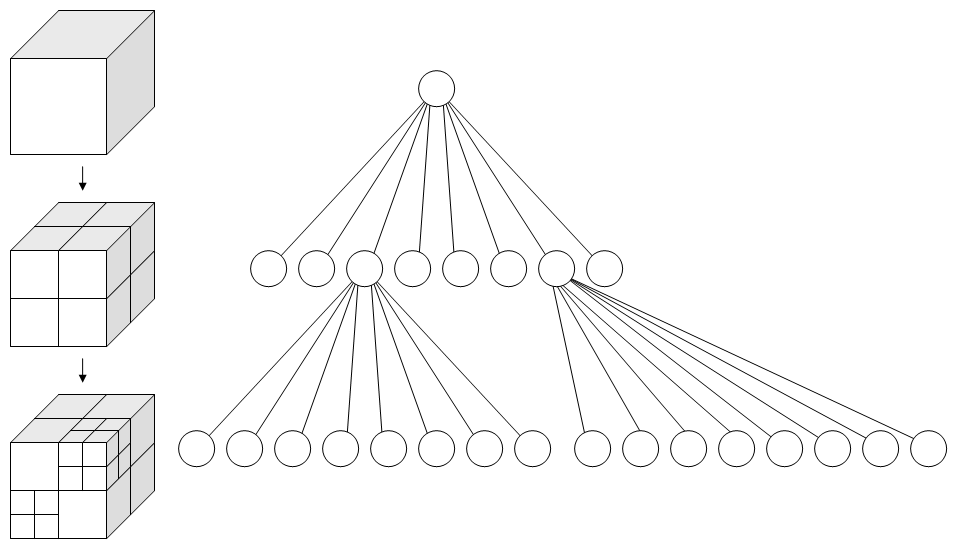
\includegraphics[width=0.8\textwidth]{../../Images/Web/Octree2.png}
  \caption{Hierarchiczny podzia� przestrzeni (na przyk�adzie Drzewa �semkowego).}
\end{figure}

Je�eli bry�a otaczaj�ca dany w�ze� przecina si� z bry�� otaczaj�c� w�ze� nale��cy do innego obiektu, to oznacza, �e wyst�puje potencjalna kolizja obiekt�w. Aby j� rozstrzygn��, nale�y sprawdzi� czy zachodz� kolizje mi�dzy bry�ami otaczaj�cymi w�z�y ni�szego rz�du. Je�li algorytm dojdzie do najni�szego rz�du hierarchii bry� otaczaj�cych, b�dzie musia� dokona� testu kolizji mi�dzy tr�jk�tami nale��cymi do tych najmniejszych w�z��w w hierarchii. Dzi�ki zastosowaniu tej techniki ju� pierwszy test mo�e wykluczy� kolizj� mi�dzy obiektami. Co wi�cej, wszystkie testy przeprowadzane w w�z�ach drzewa operuj� na prostych bry�ach geometrycznych, pozwalaj�cych na  efektywne sprawdzenie czy zachodzi kolizja. Dopiero test najni�szego rz�du wymaga badania kolizji mi�dzy tr�jk�tami, jednak�e jest ich na tym poziomie tylko od kilku do kilkunastu dla ka�dego z w�z��w.

Projektuj�c detektor, warto si� r�wnie� zastanowi�, jak wielk� precyzj� wykrywania kolizji wymaga nasza symulacja. Prawdopodobnie mo�emy ca�kowicie zrezygnowa� z testowania kolizji mi�dzy tr�jk�tami, gdy� wystarczy nam przybli�enie zapewnione przez hierarchi� bry� otaczaj�cych.

\subsection{Wyb�r obiekt�w mog�cych kolidowa�}

Z�o�ona scena 3d mo�e sk�ada� si� z bardzo du�ej ilo�ci obiekt�w. Obiekt poruszaj�cy si� np. na scenie rozgrywaj�cej si� w mieszkaniu mo�e wej�� w kolizj� z du�� ilo�ci� obiekt�w. Mog� to by� zar�wno drobne modele przedstawiaj�ce np. ksi��ki, ale te� obiekty znaczniejszych rozmiar�w przedstawiaj�ce meble i �ciany. Sprawdzanie czy poruszaj�cy si� obiekt wchodzi w kolizj� z wszystkim modelami w scenie niepotrzebnie mno�y ilo�� przeprowadzanych test�w, wp�ywaj�c na znaczne obni�enie szybko�ci detekcji kolizji. Je�li posta� znajduje si� w kuchni, to niema najmniejszego sensu sprawdzanie, czy przypadkiem nie zderzy�a si� z wann� mieszcz�c� si� na drugim ko�cu mieszkania. W celu wyeliminowania takich zb�dnych test�w stosuje si� techniki podzia�u przestrzeni.

Najbardziej uniwersalnym sposobem podzia�u przestrzeni jest zastosowanie drzewa BSP (Binary Space Partitioning - Binarny Podzia� Przestrzeni). Ka�dy w�ze� takiego drzewa dzieli opisywan� przez siebie przestrze� na dwie podprzestrzenie le��ce po przeciwnych stronach pewnej hiperp�aszczyzny. Drzewo takie mo�na zastosowa� do podzia�u przestrzeni o dowolnej wymiarowo�ci. Pozwala ono na bardzo szybkie odrzucenie obiekt�w znajduj�cych si� poza rozpatrywan� podprzestrzeni�.

\begin{figure}[h]
  \centering
  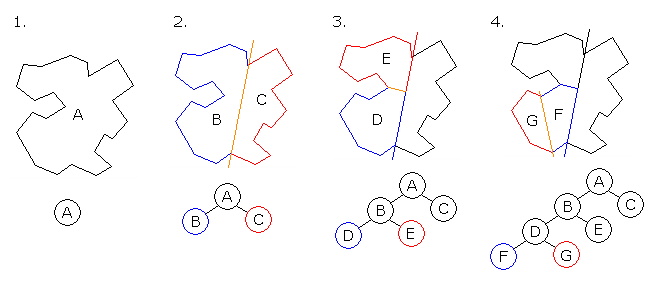
\includegraphics[width=0.8\textwidth]{../../Images/Web/Binary_space_partition.png}
  \caption{Drzewo Binernego Podzia�u Przestrzeni.}
\end{figure}

Drzewo BSP dobrze nadaje si� do opisu zamkni�tych pomieszcze�, jednak�e otwarte przestrzenie lepiej opisuj� drzewa �semkowe (lub czw�rkowe dla przestrzeni dwuwymiarowych). Drzewa takie polegaj� na otoczeniu sceny sze�cianem, kt�ry jest nast�pnie dzielony na osiem mniejszych sze�cian�w. Podzia� taki zag��bia si� rekurencyjnie, a� do osi�gni�cia ustalonego kryterium - zadanej g��boko�ci lub minimalnej ilo�ci obiekt�w w minimalnym sze�cianie. Obiekt przypisywany jest do minimalnego sze�cianu w kt�rym mo�e si� pomie�ci� oraz wewn�trz kt�rego znajduje si� jego �rodek ci�ko�ci. Wybieraj�c obiekty kt�re mog� wej�� w kolizj� z danych modelem, nale�y sprawdzi� wszystkie obiekty znajduj�ce si� w jego sze�cianie (a wi�c i w jego sze�cianach ni�szych rz�d�w) oraz s�siednie sze�ciany. W praktyce sprawdzaj�c sze�ciany s�siaduj�ce, wystarczy przejrze� te le��ce po stronie rosn�cych wsp�rz�dnych - kolizje z pozosta�ymi s�siadami zosta�y sprawdzone podczas badania kandydat�w dla obiekt�w nale��cych do tamtych podprzestrzeni.


\section{Symulacja fizyki}

Posiadaj�c wiedz� o si�ach oddzia�uj�cych na obiekty oraz kolizjach do kt�rych dosz�o, mo�na przej�� do symulacji ruchu. Przyk�adowym podej�ciem mo�e by� otwarcie podr�cznika do fizyki i�zastosowanie przedstawionych w nim wzor�w opisuj�cych ruch.

Stosuj�c opis dynamiczny na poziomie modelu jako ca�o�ci, nale�a�oby uwzgl�dni� w algorytmie takie wielko�ci jak pozycja, pr�dko��, masa obiektu, a tak�e dzia�aj�ce na� si�y. Model taki jest w najprostszym przypadku cia�em sztywnym, nie mo�na wi�c r�wnie� zapomnie� o opisuj�cych ruch obrotowy momencie bezw�adno�ci oraz momencie si�y. Gdy zechcemy symulowa� cia�a odkszta�calne, takie jak materia�y, powierzchnie elastyczne, b�d� ro�liny, nasz algorytm rozro�nie si� jeszcze bardziej.

\subsection{Ca�kowanie Verlet'a}

Alternatywne podej�cie do symulacji zachowania si� cia� fizycznych zastosowano po raz pierwszy w grze \textit{Hitman: Codename 47}. Rozwi�zanie to przedstawi� w swym artykule dyrektor do spraw  bada� i rozwoju w firmie IO Interactive, Thomas Jakobsen \cite{JAKOB}. Polega ono na rozbiciu obiektu na zbi�r punkt�w materialnych i rozpatrywaniu ruchu ka�dego punktu osobno. Ponadto, w celu poprawy stabilno�ci algorytmu, zrezygnowano z przechowywania pr�dko�ci cz�steczki. W efekcie ka�da cz�steczka opisywana jest przez cztery wielko�ci fizyczne: pozycj�, pozycj� w poprzedniej klatce (wymagana do wyliczenia faktycznej pr�dko�ci), mas� oraz wypadkowe przy�pieszenie cz�steczki. Ca�y opis ruchu pojedynczego punktu materialnego sprowadza si� do nast�puj�cego wzoru:
\begin{equation}
x_{t+1} = 2 * x_{t} - x_{t-1} + a * \Delta t^{2}
\end{equation}
Podej�cie to nazywa si� ca�kowaniem Verlet'a i jest szeroko wykorzystywane w symulacji dynamiki molekularnej. Pr�dko�� cia�a zaszyta jest w tym wzorze pod postaci� r�nicy po�o�enia w w sta�ej jednostce czasu:  $x_{t} - x_{t-1}$.

\subsection{Nak�adanie ogranicze� na punkty materialne}

Za pomoc� chmury niezale�nych punkt�w materialnych, mo�emy opisa� co najwy�ej silnik cz�steczkowy. Je�li jednak chcieliby�my by nasze cz�steczki opisywa�y bardziej z�o�one cia�a, musimy na�o�y� na nie ograniczenia.

\begin{figure}[h]
  \centering
  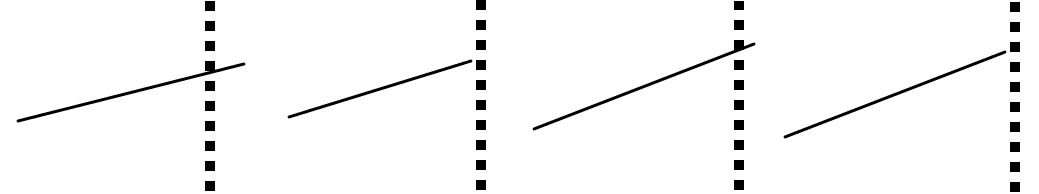
\includegraphics[width=1\textwidth]{../../Images/SDM_constraint.png}
  \caption{Kolejne kroki procesu spe�niania ogranicze�.}
\end{figure}

W podej�ciu przedstawionym przez Jakobsena zbi�r ogranicze� na�o�onych na system spe�niany jest poprzez relaksacj�. Proces ten postaram si� opisa� na przyk�adzie dw�ch cz�steczek opisuj�cych sztywny pr�t. Odleg�o�� mi�dzy tymi cz�steczkami musi by� sta�a. Dodatkowo pr�t nie powinien przebi� �adnego innego obiektu. Na rysunku 3a widzimy sytuacj� w kt�rej to drugie ograniczenie zosta�o naruszone. Pr�t przechodzi przez �cian� reprezentowan� przez przerywan� lini�. W pojedynczym kroku symulacji, przez zadan� ilo�� iteracji, silnik b�dzie po kolei spe�nia� ka�de z ogranicze�. W ramach spe�niania tego ograniczenia, punkt kt�ry przebi� �cian� zosta� rzutowany na poprawn� pozycj�. Spe�nienie tego ograniczenia naruszy�o jednak ograniczenie drugie � cz�steczki znalaz�y si� zbyt blisko siebie (rys. 3b). Aby spe�ni� ten warunek, punkty musz� zosta� rozsuni�te � spowoduje to jednak ponowne przebicie �ciany (rys. 3c). W kolejnych iteracjach relaksacji ograniczenia b�d� naruszane w coraz mniejszym stopniu, a� w ko�cu wszystkie zostan� spe�nione.

Co interesuj�ce, w pojedynczej klatce symulacji nie musimy doprowadza� do spe�nienia wszystkich ogranicze�. Korygowanie pozycji cz�steczek mo�e by� kontynuowane w kolejnych klatkach.

\subsection{Symulacja cia� odkszta�calnych}

Aby opisa� zachowanie cia� odkszta�calnych, takich jak ubrania b�d� ro�liny, wystarczy ka�dy wierzcho�ek siatki modelu symulowa� jako pojedynczy punkt materialny. Na punkty te powinny zosta� na�o�one warunki zachowania sta�ej odleg�o�ci pokrywaj�ce si� z kraw�dziami tr�jk�t�w siatki. Dla uzyskania �adnej animacji takich cia� wystarczy tylko pojedyncza iteracja relaksacji na klatk� symulacji.

\subsection{Symulacja cia� sztywnych}

Najprostszym sposobem na przedstawienie cia�a sztywnego, jest zastosowanie takiego samego podej�cia jak dla cia� odkszta�calnych, lecz z na�o�eniem ogranicze� sta�ej odleg�o�ci na wszystkie pary wierzcho�k�w. Wydajniejszym podej�ciem jest jednak opisanie ca�ego cia�a sztywnego z wykorzystaniem jedynie czterech punkt�w materialnych po��czonych ograniczeniami sta�ej odleg�o�ci. Ustawienie tych cz�stek w konfiguracji np. czworo�cianu foremnego zapewni 6 stopni swobody, a wi�c dok�adnie tyle, ile posiada cia�o sztywne. W zale�no�ci od sposobu ustawienia cz�steczek, cia�o b�dzie mia�o r�ny moment bezw�adno�ci.

Jedynym problemem jaki pozostaje do rozwi�zania jest roz�o�enie  si�y przy�o�onej do pewnego punktu (np. punktu kolizji) na si�y sk�adowe dzia�aj�ce na poszczeg�lne cz�steczki. Dowolny punkt w przestrzeni mo�e by� przedstawiony jako liniowa interpolacja punkt�w materialnych kt�re symulujemy. Korzystaj�c z parametr�w tej interpolacji mo�emy dokona� operacji odwrotnej by proporcjonalnie roz�o�y� si�� pomi�dzy wszystkie cz�steczki.

\subsection{Fizyka szkieletu}

Silnik oparty na ca�kowaniu Verlet'a bardzo dobrze nadaje si� r�wnie� do symulowania fizyki cia� posiadaj�cych szkielet. Wystarczy stawy przedstawi� jako punkty materialne, a ko�ci jako warunki zachowania sta�ej odleg�o�ci. Dodatkowo nale�y doda� ograniczenia k�towe, kt�re uniemo�liwi� 'wykr�canie staw�w'. Dobrym rozwi�zaniem ograniczaj�cym przecinanie si� ko�ci postaci (silnik fizyczny rozpatruje tylko kolizje z innymi modelami), jest dodanie warunk�w minimalnej odleg�o�ci pomi�dzy takimi stawami jak kolana i kostki st�p.

\begin{figure}[h]
  \centering
  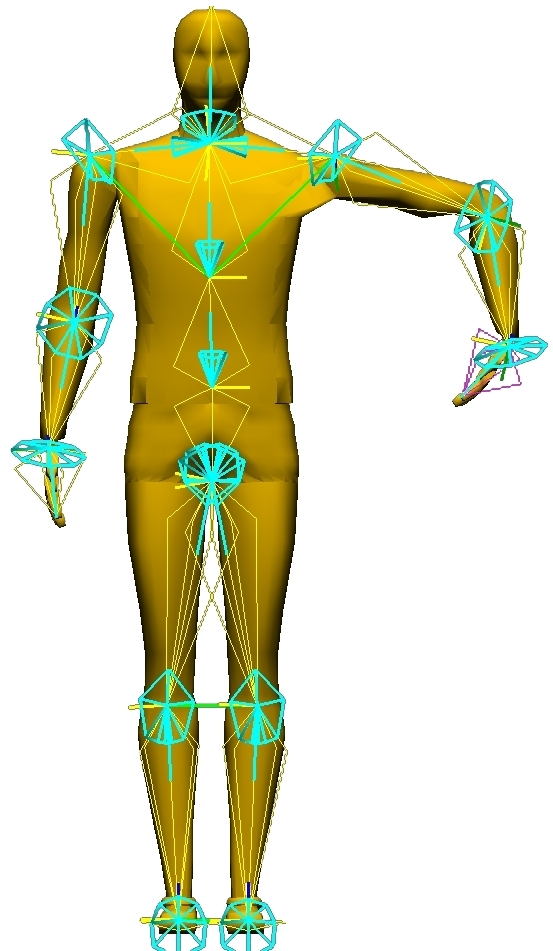
\includegraphics[width=0.4\textwidth]{../../Images/Gameplay/editor_constraints.jpg}
  \caption{Szkielet z na�o�onymi ograniczeniami k�towymi.}
\end{figure}

W przeciwie�stwie do innych typ�w obiekt�w, cz�steczki reprezentuj�ce stawy musz� by� nap�dzane nie tylko samym procesem ca�kowania Verlet'a, ale r�wnie� przez zewn�trzne �r�d�a ruchu, takie jak animacje przygotowane przez artyst�w. Rozwi�zaniem problemu mo�e by� algorytm, kt�ry b�dzie miesza� zewn�trzn� animacj� z wynikiem dzia�ania ca�kowania. Waga ka�dego ze �r�de� powinna by� zmienna. Je�li np. model zostanie uderzony z du�� si��, to kontrol� powinien przej�� silnik Verlet'a. W pozosta�ych sytuacjach wi�ksz� wag� powinno si� przyk�ada� do 'woli' postaci, czyli animacji narzuconych przez logik� gry.

\begin{thebibliography}{99}

\bibitem[DG02]{RR4488}
Olivier Devillers and Philippe Guigue, 2002\\
'Faster triangle-triangle intersection tests'\\
http://www.inria.fr/rrrt/rr-4488.html

\bibitem[Jak03]{JAKOB}
Thomas Jakobsen, 2003\\
'Advanced character physics'\\
http://www.gamasutra.com/resource\textunderscore guide/20030121/jacobson\textunderscore 01.shtml

\bibitem[Wik]{WIKI_CD}
Wikipedia\\
'Collision detection'\\
http://en.wikipedia.org/wiki/Collision\textunderscore detection

\end{thebibliography}

%%\nocite{*}
%%\bibliography{sdm2-esej}

\end{document}

